\documentclass[notitlepage,12pt]{article}
\usepackage{fancyvrb, verbatim, listings}                                  % Various for inserting/hosting code
\usepackage{setspace}                                                      % Space between lines (customisable)
\onehalfspacing
\usepackage[margin=2.54cm]{geometry}                                       % Set margins (standard is 2.54cm)
\usepackage[UKenglish]{babel}                                              % Set default language
\usepackage[UKenglish,cleanlook]{isodate}                                  % Set default date and date display
%\usepackage{palatino, microtype}                                          % Change font and minor spacings to look nicer
%% Packages to use:
% Tables + figures
\usepackage{graphicx}                                                      % control over the import of graphics
\usepackage[table,dvipsnames]{xcolor}                                      % Define tables (with colour control)
\usepackage{float}                                                         % Control over graphics + tables float
\usepackage{booktabs}                                                      % caption graphics + tables (with name in bold)
\usepackage[labelfont=bf]{caption}                                         % caption graphics + tables (with name in bold)
\usepackage{subcaption}                                                    % subcaption graphics + tables
\usepackage{tikz}                                                          % Draw graphs inline, guide: https://sites.google.com/site/kochiuyu/Tikz
\newenvironment{ctikzpicture}{                                             % center the graphs by default 
    \begin{center}\begin{tikzpicture}}{
    \end{tikzpicture}\end{center}}
\usepackage[shortlabels]{enumitem} \setlist[enumerate]{leftmargin=0pt}     % Customisable lists
% Maths + numbers
\usepackage{mathtools}                                                     % Various maths functions
\usepackage{amsmath}                                                       % Various maths functions
\usepackage{amssymb}                                                       % Various maths functions
%\usepackage{siunitx}                                                      % Formalise use of units and numbers among text
\usepackage{centernot}                                                     % center \not usage
\DeclareMathOperator{\eps}{\varepsilon}                                    % epsilon short hand shortcut
\DeclareMathOperator{\st}{\text{ s.t. }}                                   % "such that" short hand shortcut
\DeclareMathOperator{\then}{\text{ then }}                                 % "then" in equation shortcut
\DeclareMathOperator{\ifeq}{\text{ if }}                                   % "if" in equation shortcut
\DeclareMathOperator{\oreq}{\text{ or }}                                   % "or" in equation shortcut
\DeclareMathOperator{\all}{,\; \forall}                                    % all with spacing in equation shortcut
\DeclareMathOperator{\N}{\mathbb{N}}                                       % N, natural number, shortcut
\DeclareMathOperator{\R}{\mathbb{R}}                                       % R, real number, shortcut
\newcommand{\fakeslant}[1]{\pdfliteral{1 0 0.167 1 0 0 cm}#1\pdfliteral{1 0 -0.167 1 0 0 cm}}
\renewcommand{\vec}[1]{\mathbf{\fakeslant{#1}}}                            % vector notation for unit shortcut
\newcommand{\mat}[1]{\mathbf{\fakeslant{#1}}}                              % matrix notation for unit shortcut
\newcommand{\Prob}[1]{\ensuremath{\mathbb{P}\left( #1 \right)}}            % SHortcut for probability notation
\newcommand{\Probgiven}[2]{\ensuremath{\mathbb{P}\left( #1 \, \middle\vert \, #2 \right)}}            % SHortcut for probability notation, given
\newcommand{\E}[2][]{\ensuremath{\mathbb{E}_{#1} \left[ #2 \right]}}       % Expectation (with optional subscript) shortcut
\newcommand{\Egiven}[3][]{\ensuremath{\mathbb{E}_{#1} \left[ #2 \, \middle\vert \, #3 \right]}}       % Expectation (with optional subscript) shortcut
\newcommand{\Var}[2][]{\ensuremath{\text{Var}_{#1} \left( #2 \right)}}     % Variation (with optional subscript) shortcut
\newcommand{\Cov}[1]{\ensuremath{\text{Cov} \left( #1 \right)}}            % Covariance (with optional subscript) shortcut
\newcommand{\1}[1]{\ensuremath{\mathbb{1}\left( #1 \right)}}               % SHortcut for indicator function
\newcommand{\diff}[2][]{\ensuremath{\frac{d#1}{d#2}}}                      % SHortcut for differential fraction as a function
\newcommand{\partialdiff}[2][]{\ensuremath{\frac{\partial#1}{\partial#2}}} % SHortcut for partial differential fraction as a function
\newcommand{\converge}[1]{\xrightarrow{ #1 \to\infty}}                     % SHortcut for convergence arrow
\newcommand{\ans}{\par \textbf{Answer:} }                                  % SHortcut to start answer of a question
% Citations 
\usepackage[longnamesfirst]{natbib}                                        % Reference manager
\usepackage{hyperref}                                                      % Allow for links across the text, with colour options
\hypersetup{colorlinks=true, linkcolor=blue, citecolor=blue, filecolor=magenta, urlcolor=blue}
% Top of pages
\usepackage{fancyhdr}
\pagestyle{fancy}
\lhead{The Rise in Returns to Skill?}
\rhead{Senan Hogan-Hennessy}
% Author
\author{Senan Hogan-Hennessy\footnote{This paper was completed in accordance with requirements for the Pomona College Department of Economics Senior Seminar, Spring 2018.
I am grateful for the comments and guidance of Michael Kuehlwein, Pomona College Department of Economics.} \\
Senior Seminar in Economics\footnote{
  This project's Github repository, with materials for replication, is available at
  \href{https://github.com/shoganhennessy/Econ_text_data}{\nolinkurl{github.com/shoganhennessy/ECON190}}.}}

% Title
\title{The Rise in Returns to Skill? \\ \Large{A Modern Regression Analysis of Wage Inequality in the Current Population Survey}}

% Date
\date{\begin{singlespace} \normalsize{
\vfill Pomona College, Department of Economics \\
\noindent 425 N. College Ave.  \\
\noindent Claremont CA 91711   \\
\noindent May 2018}
\end{singlespace}}
%%% BEGIN %%%
\begin{document}
\maketitle
\thispagestyle{empty}

\newpage \thispagestyle{empty}
\begin{singlespace}
\noindent The Rise in Returns to Skill?  A Modern Regression Analysis of Wage Inequality in the Current Population Survey

\noindent Senan Hogan-Hennessy

\noindent Working Paper, Senior Seminar in Economics

\noindent May 2018
\end{singlespace}

% Abstract
\begin{abstract} \noindent
A wage decomposition shows the contribution of workers' observed and unobserved characteristics, and their
returns, to the distribution of income.  
Yet the estimated contributions and determinants of rising income inequality change with how wages are
econometrically modelled.
I extend the Juhn, Murphy \& Pierce (1993) decomposition to multiple econometric models, including 
modern regression methods, on the US income distribution 1980--2016.
There is a larger contribution of observed and unobserved worker characteristics 
in rising wage inequality than previous estimates suggest,
and a smaller contribution from changing returns to worker characteristics
using modern regression methods to model wages.
The analysis shows the wage decomposition's vulnerability to choice of wage model,
and discusses the further use of modern regression methods in econometric models of wages.
\end{abstract}
\vfill
\begin{singlespace}
\noindent Senan Hogan-Hennessy

\noindent Pomona College

\noindent 425 N. College Ave.

\noindent Claremont CA 91711
\end{singlespace}


\newpage
\setcounter{page}{1}
% Introduction
\noindent
Wage inequality has been rising drastically since the 1960s, possibly due to many factors.  Multiple significant studies decompose wage inequality, attributing a large portion of the rise in inequality to a rise in returns to skill and unobservable characteristics, first shown by \cite{juhn1993wage}.  The methods for wage prediction and determining observable skills are extremely important in determining this composition, and have previously only used a standard linear regression.  This paper uses modern regression techniques to expand the \cite{juhn1993wage} decomposition method to modern regression techniques.  The random forest prediction method produces more accurate estimates of wages than the standard linear regression approach, leading to a different composition of observed characteristics in explaining wage inequality.  This analysis thus shows how dependent the wage decomposition is to the exact prediction method used, an issue that has not before been examined rigorously. 

Wage inequality rose consistently from 1980, following an accelerated rise for those with at least a college degree compared to the rest of the population.  The distribution of residuals in wages rises regardless of prediction method, also becoming more unequal across the time period.  However, the modern techniques predict a less dramatic rise in inequality across the residual distribution.  Standard linear models predict that unobserved skill contributes the most of any component to rising inequality, and modern regression models attribute even more of the rise in inequality to unobserved factors.  They also exhibit a rising importance for years of education in predicting wages, with a fall in the role of gender.

The paper is structured as follows.
Section~\ref{literaturereview} surveys the current literature on wage inequality and decomposition by regression approaches.
Section~\ref{wageinequality} describes the March Current Population Survey (henceforth March CPS) data set, and trends in income inequality for the US.
Section~\ref{explaininginequality} presents the wage decomposition, and various regression prediction methods for the empirical analysis.
Section~\ref{results} presents the results of each approach.
Section~\ref{discussion} discusses the findings of the paper, with lessons to learn for studies that use predictive models and regression approaches in the study of wage inequality.
Section~\ref{conclusion} concludes.

% LIT REVIEW
\section{Literature Review}
\label{literaturereview}
Wage inequality has increased dramatically since the 1950's in the US.  Many studies in labour economics attribute this rise in inequality to a rise in the returns to skill.  Across other subfields of economics, however, there are multiple factors that also explain rising inequality, ranging from rise in market power \citep{furman2015firm}, to de-unionisation and supply and demand shocks \citep{DML95}, to ``skill-biased technological change'' \citep{acemoglu1998new,acemoglu2002technical}.  The literature that attributes a large percentage of the rise in wage inequality to an increase in returns to skill mainly relies on regression approaches pioneered by \cite{mincer1958investment,mincer1974schooling}.

\subsection{Wage Decomposition and Ordinary Least Squares}

The Mincer wage equation applies the standard ordinary least squares (OLS) regression method is used to predict wages by simple function of potential experience and years of education.  This method was noted as being successful in explaining wages and wages inequality, while maintaining an intuitive basis, and has become a benchmark model in labour economics.  \cite{juhn1993wage} showed a drastic rise in wage inequality between 1963 and 1989, using the March CPS -- a representative data set for the US population.  The analysis extends the decomposition method of \cite{jmp2011} that focuses on wage predictions and residuals in a few standard regressions, showing the role of unobserved skills.  The methods make a few notable assumptions, and crucially show the Mincer wage equation produces much worse estimates for wages (i.e. higher errors) in the late 1980's that did in earlier decades.  The approach has some notable criticisms: \cite{yun2009wage} questions the validity of using the change in distribution of residuals to explain discrimination in the decomposition methods of \cite{jmp2011,juhn1993wage}, while \cite{lemieux2006increasing} attributes the rise in wage inequality to a secular increase in experience and education, attributing the results of \cite{juhn1993wage} to composition factors and noisy data.

Today the Mincer wage equation is noted as in need of adjustments to capture changes in the US economy and acknowledge advances in empirical labour economics.  \cite{lemieux2006mincer} proposes functional adjustments to accommodate changes in the economic relationship between years of education and wages seen in wage data until the 1990's.  However, the US economy is very different today than it was in the 1950's, especially in terms of size, complexity and technology.  Today, supply chains are increasingly complicated and dependent on global markets, entire industries have risen and fallen with ramifications for structural employment, and the Internet has revolutionised many sectors of the economy.  Labour economic studies that use the original Mincer wage function to predict wages in the modern economy do not fully acknowledge the rise in complexity or resulting changes in the determinants of wages.  That is the simple linear equation may only capture changes through an increase in estimated returns to education, experience and potential experience, yet may not acknowledge any change in the composition or functional form of them and other variables in determining wages.  Modern regression approaches provide a viable option to better address these empirical problems.

\subsection{Modern Regression Techniques}

Regression practices have advanced tremendously in the last few decades, and since Dr Jacob Mincer began modern labour economics as a field.  The original Mincer wage equation provides a method for intuitive prediction of wages, but provides an overly simplified version of the story.  There are many variables -- observed, unobserved, or even unobservable -- with possible explanatory power for wages in the US economy.  There are also many ways in which these variables relate to wages (linear or non-linear), and which have changed from those in previous decades.  This problem can not be completely fixed by a simple adjustment, as noted by \cite{lemieux2006increasing}.  These issues bring into question the robustness of only using the simple OLS approach in analyses that require prediction of wages with given data.

Regression by machine learning practices provide a viable avenue to expand the literature, and more robustly estimate returns to skill in the US economy.  For example, a regression tree is a completely different form of regression than OLS and common econometric methods.  The process involves building a decision tree by minimising an error function by splitting on available variables, relaxing any linear restrictions on the model.  Bootstraps of data are used to form a random forest model, with extremely high power for prediction with less problems of over-fitting data \citep{breiman2001random}.  Labour economics  has, however, been slow to use such techniques in empirical studies.  \cite{belloni2011high} and \cite{abadie2017risk} develop novel prediction techniques, and test their properties by predicting wages in the March CPS.  \cite{chalfin2016productivity} demonstrate the benefit of predictive power of tree-based machine learning methods in productivity of public sector workers.  Gains in predictive power from these methods are noted as ``large both absolutely and relative to those from interventions studied by standard causal analyses in microeconomics.''

\section{Wage Inequality in the US}
\label{wageinequality}
\subsection{Data}
The analysis of this paper is conducted on 35 years of wage and demographic information for individuals taken from the March Annual Social and Economic Supplement of the Current Population Survey, commonly referred to as the March CPS.  The 35 years span 1980--2016 (without 2008), with data referring to the 12 months preceding the March survey.  Uniform extracts of the March CPS are taken, in full, from publicly available hosting by the Centre for Economic Policy Research \nocite{center} (Version 1.0, 2016).

\begin{table}[!htbp] \centering 
  \caption{Summary Statistics, 1980-2016} 
  \label{tab:summarystats}
    \begin{tabular}{@{\extracolsep{5pt}}lccccc} \\[-1.8ex]\hline 
\hline \\[-1.8ex]
Statistic & \multicolumn{1}{c}{Observations} & \multicolumn{1}{c}{Mean} & \multicolumn{1}{c}{St. Dev.} & \multicolumn{1}{c}{Min} & \multicolumn{1}{c}{Max} \\ 
\hline \\[-1.8ex] 
Hourly wage, \$ & 2,185,520 & 25.15 & 149.73 & 7.250 & 94,963.63 \\  
Annual income, \$ & 2,185,520 & 50,426& 50,975 & 4,060 & 1,848,079 \\ 
Age & 2,185,520 & 39.612 & 11.671 & 18 & 65 \\ 
Years of education & 2,185,520 & 13.7 & 2.7 & 0 & 22 \\ 
Female & 2,185,520 & 0.46 & 0.50 & 0 & 1 \\ 
Race & 2,185,520 & 1.289 & 0.752 & 0 & 3 \\ 
Married & 2,185,520 & 0.640 & 0.480 & 0 & 1 \\ 
Rural & 2,185,520 & 0.205 & 0.404 & 0 & 1 \\ 
Suburb & 2,185,520 & 0.381 & 0.486 & 0 & 1 \\ 
Central city & 2,185,520 & 0.237 & 0.426 & 0 & 1 \\ 
Self employed & 2,185,520 & 0.003 & 0.051 & 0 & 1 \\ 
\hline \\[-1.8ex] 
\end{tabular} 
\end{table}
Analysis of inequality refers to wage information at the hourly level, defined as annual earnings divided by annual hours worked,\footnote{Weekly hours worked times by amount of weeks worked in a year.} and at the annual level, defined as total income in the 12 months preceding, as specified.  Wages are adjusted according to the CPI Research Series Using Current Methods (CPI-U-RS), set to 2015 dollars.\footnote{These specifications for wages are provided in full by the CEPR Extracts.}  The sample is restricted to full-time workers, both male and female,\footnote{Whereas \cite{juhn1993wage} analyse only men's wages in order to remove effects of rising women's labour force participation.  This study however considers a later time period when women participation is relatively similar and so includes women.} making at least the 2015 hourly federal minimum wage (\$7.25) between ages 18 and 65.  The total number of observation is 2,185.520, which is extremely large (even when treated in year increments) and so is adequately large to apply modern big-data regression methods.\nocite{varian2014big}  Observations from the year 2008 are excluded due to sample size problems.\footnote{2008 has remarkably few observations that fit the above criteria.  Specifically the years 2007 and 2009 have 77,907 and 75,175 observations respectively, whereas 2008 has 13,720.  This led to unusually high averages and quantiles for wages in the year 2008 compared to years either side -- counter-intuitively given economic conditions -- so that this year is excluded in analysis.}  See Table~\ref{tab:summarystats} for summary statistics for real hourly and annual wage, age, years of education, and proportion female for the sample, and a collection of variables used in the prediction methods (explained in section 4.1).


\subsection{Rising Inequality}
\begin{figure}[H]
  \centering
  \caption{Indexed Real Hourly Wage by Percentile, 1980-2016.}
  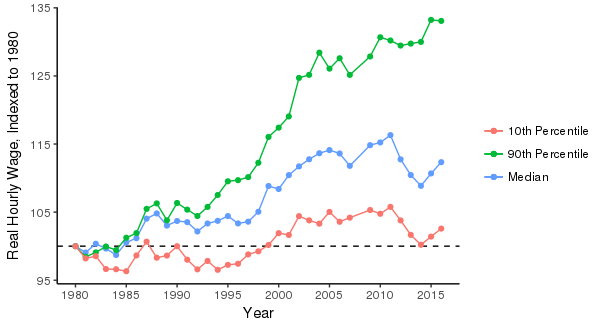
\includegraphics[width=0.8\textwidth]{figures/Ineq_graph.png}
  \label{fig:wages_percentile}
\end{figure}
\begin{figure}[b]
  \centering
  \caption{Ratio of Wage Between 90th and 10th Percentiles, 1980-2016.}
  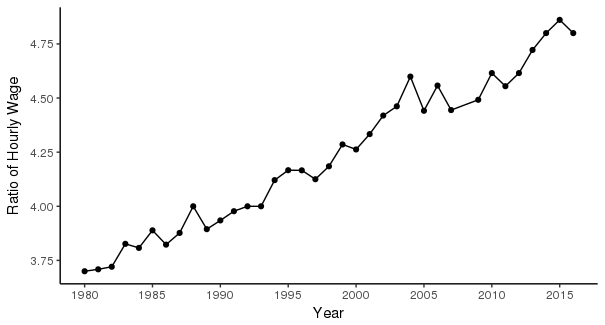
\includegraphics[width=0.6\textwidth]{figures/Ratio_plot1.png}
  \label{fig:ratios_percentile}
\end{figure}
Figure~\ref{fig:wages_percentile} presents the 10th, 50th and 90th percentile of the hourly wage distribution 1980--2016.  Each series is indexed to 1980 (so that each is assigned a value of 100 in 1980) for comparison between the groups and visualisation of their respective changes since 1980.  The 90th percentile of he wage distribution saw a mild increase in income from 1980 until 1990, followed by a rapid rise until the mid-2000s.  The median of the income distribution steadily increased until 2007 at a lower rate than the 90th percentile, while the 10th percentile saw a general stagnation across the time period, including any gains made over the 2000s vanishing in the years following 2010.  Figure~\ref{fig:ratios_percentile} presents the ratio between the 90th and 10th percentile of the hourly wage distribution 1980--2016.  The series shows a clear and persistent increase for the 36 year period, following a trend documented for preceding decades in previous research.

\begin{figure}[H]
  \centering
  \begin{subfigure}{.5\textwidth}
    \centering
    \caption{Hourly Wage.}
    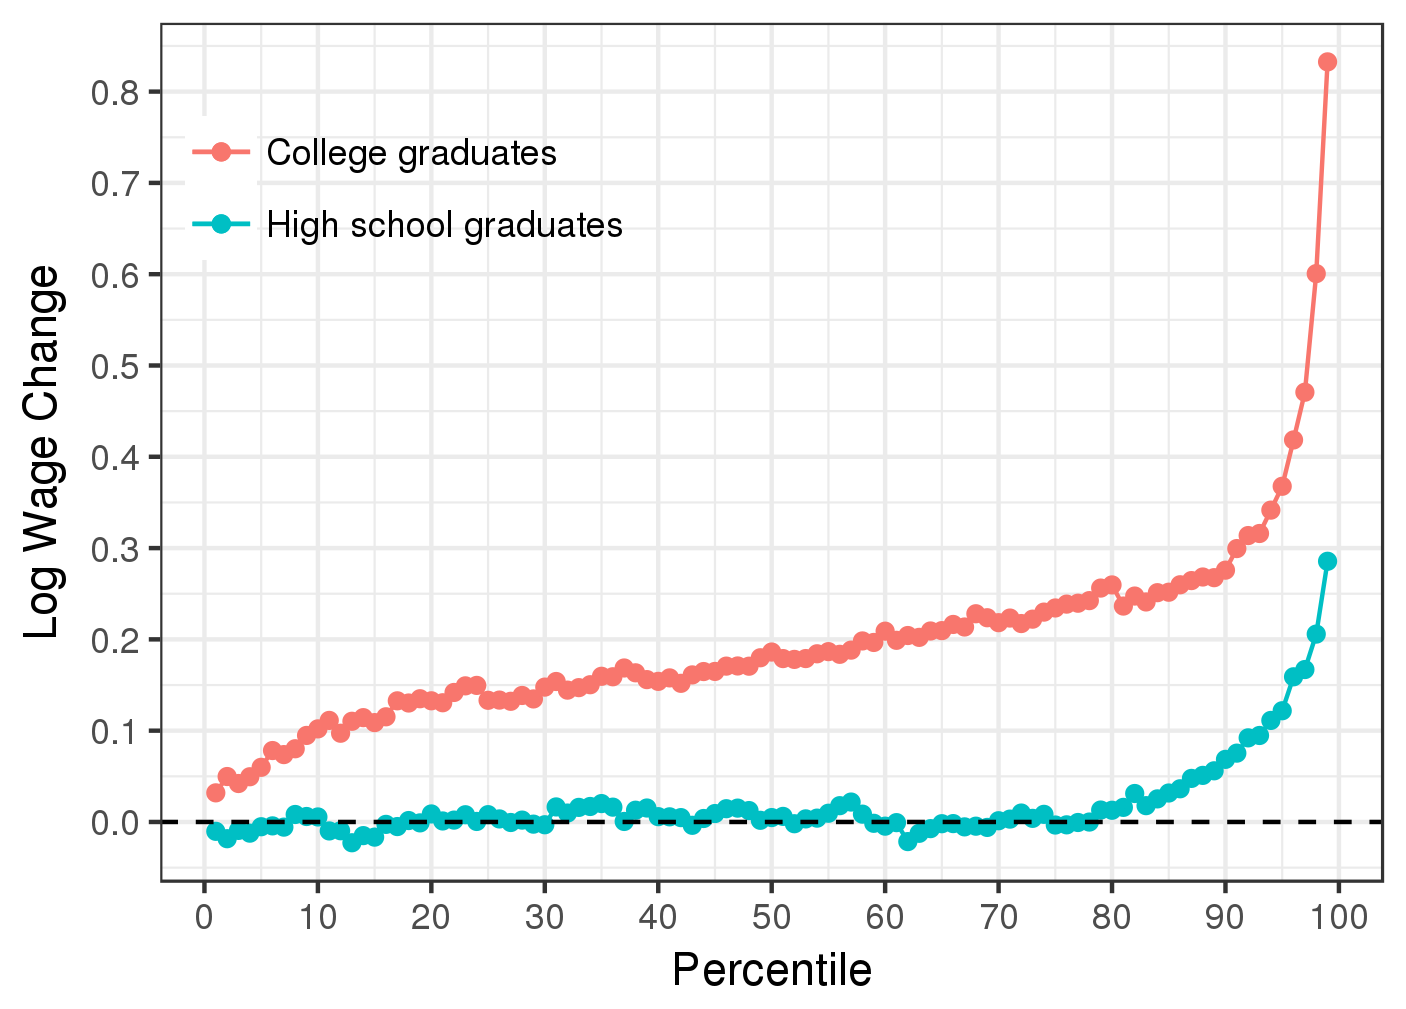
\includegraphics[width=\textwidth]{figures/hour_wage_change.png}
  \end{subfigure}%
  \begin{subfigure}{.5\textwidth}
    \centering
    \caption{Annual Income.}
    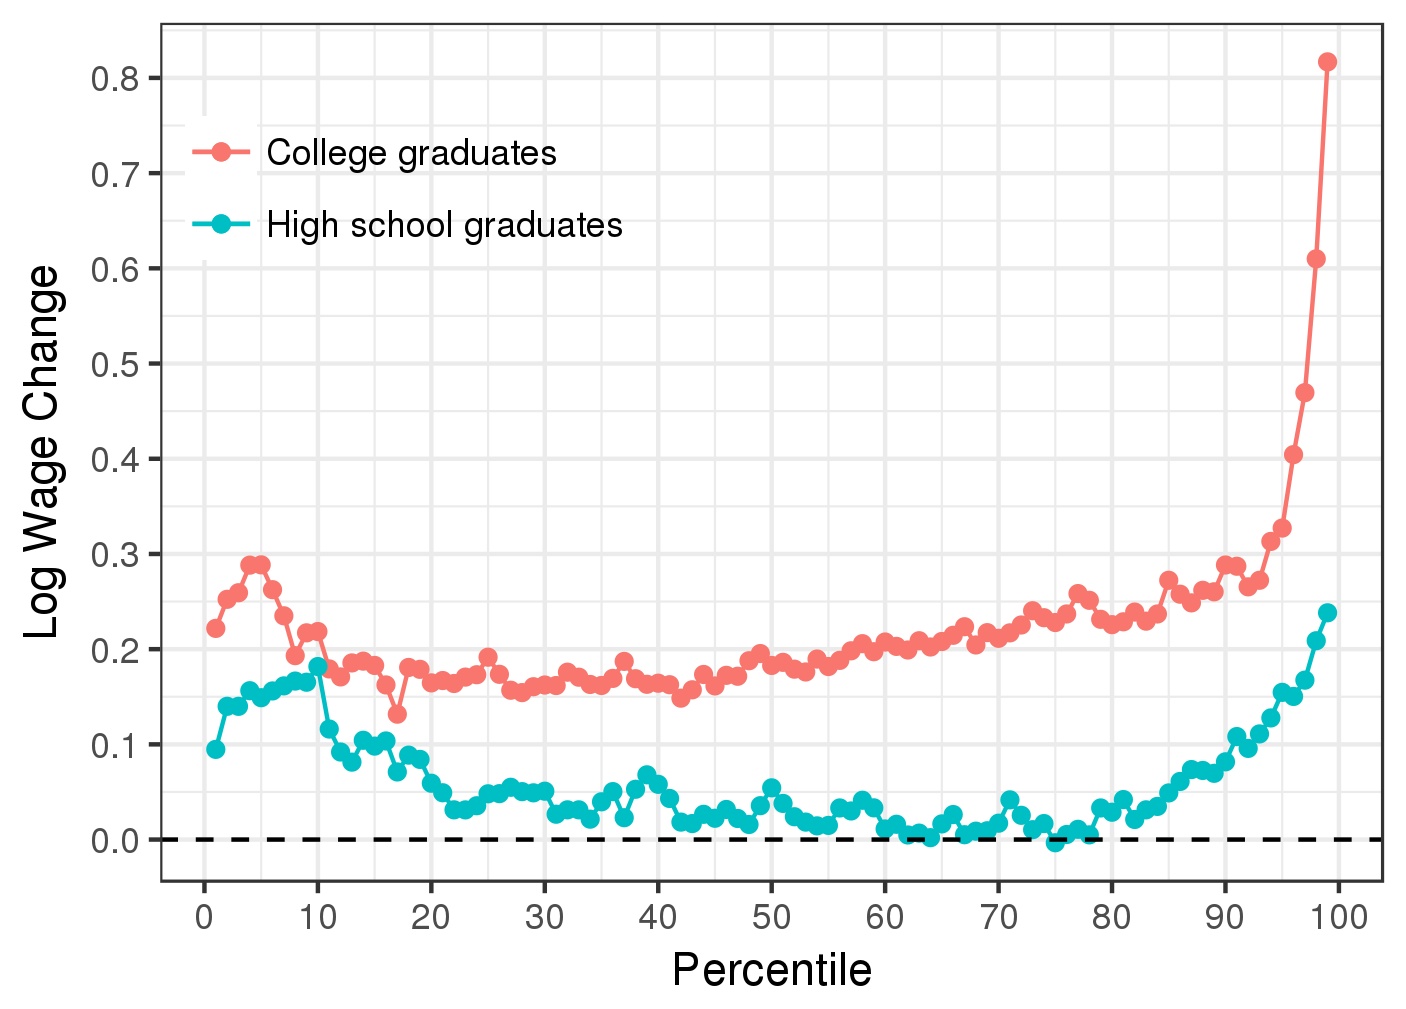
\includegraphics[width=\textwidth]{figures/annual_wage_change.png}
  \end{subfigure}
  \caption{Wage Change by Percentile, 1980--2016.}
  \label{fig:wagechange_percentile}
\end{figure}
Figure~\ref{fig:wagechange_percentile} shows the log wage change across the income distribution (percentiles 1 to 99) for college graduates and high school graduates.\footnote{3 years groupings are used for 1980 and 2016, i.e. 1980-1983 vs 2013-2016, to limit variation.}  High school graduates in the bottom 80\% saw no change in hourly wage,\footnote{Likely due to sample restrictions limiting samle to an income of a minimum wage full-time worker.} and only saw increase in annual income for the bottom 10\%.  College graduates's hourly wage increase sees a linear trend for percentile with the 10th percentile increasing by around 0.1 log points and the 90th by around 0.3 log points, with a similar yet (but not as steep) linear trend for annual income.  Above the 10th percentile both measures of income rose by many multiple of any other percentile, showing a large increase in income at the top of the income distribution.  \cite{juhn1993wage} document the linear rise in the income distribution between the 10th and 90th percentiles between 1970 and 1985.  The rise in wage inequality since then has laregly been driven by gains in income \textit{above} the 90th percentile, however.

\section{Explaining Wage Inequality}
\label{explaininginequality}
Wage Inequality has risen significantly since 1980.  The role that changing returns to skills, observable or unobservable, plays in explaining this rising in inequality is not so clear cut.  Equation~\eqref{eqn:standard} presents a standard linear regression that aims to decompose wage inequality in the form of a standard wage equation. 
\begin{equation}
  \label{eqn:standard}
  Y_{it} = \mathbf{X}_{it}\beta_t + \varepsilon_{it}
\end{equation}
$Y_{it}$ represents the log weekly wage for individual $i$ in year $t$, $\mathbf{X}_{it}$ a vector of observable characteristics and $\beta_t$ the vector of coefficients representing returns to observable skills. $\varepsilon_{it}$ is the standard residual, the component for wages that are not otherwise explained by specified variables in the given regression method (unobserved characteristics).  The residual may be specified in terms of a distribution, in equation~\eqref{eqn:errors}, where $F_{it}(. | \mathbf{X}_{it})$ is the cumulative density function for residuals of individuals with observed characteristics $\mathbf{X}_{it}$ in year $t$.
\begin{equation}
  \label{eqn:errors}
  \varepsilon_{it} = F_{t}^{-1}(\theta_{it} | \mathbf{X}_{it})
\end{equation}

Decomposition of wage inequality involves attributing changes in inequality to three factors across time: changes in observable characteristics (i.e. changes in $\mathbf{X}_{it}$), changes in returns to observable characteristics (i.e. changes in $\beta_t$), and changes in unobserved characteristics and their returns (i.e. changes in $\varepsilon_{it}$).  \nocite{autor200914}To demonstrate this decomposition define $\beta$ to be the returns to observable characteristics and $F(. | \mathbf{X}_{it})$ the cumulative distribution for residuals across a reference time period, here 1980--1985, so that neither varies year on year.  $Y_{it}^1$, $Y_{it}^2$, $Y_{it}^3$ are then defined as follows.
\begin{gather}
  \label{eqn:decomposition_Y1}
  Y_{it}^1 = \mathbf{X}_{it}\bar{\beta} + \bar{F}^{-1}(\theta_{it} | \mathbf{X}_{it}) \\
  \label{eqn:decomposition_Y2}
  Y_{it}^2 = \mathbf{X}_{it}\beta_t + \bar{F}^{-1}(\theta_{it} | \mathbf{X}_{it}) \\
  \label{eqn:decomposition_Y2}
  Y_{it}^3  = \mathbf{X}_{it}\beta_t + F_{t}^{-1}(\theta_{it} | \mathbf{X}_{it}) = \mathbf{X}_{it}\beta_t + \varepsilon_{it}  = Y_{it}
\end{gather}
$Y_{it}^1$ is the distribution of wages under fixed returns to observable characteristics, so that $\bar{F}^{-1}(. | \mathbf{X}_{it})$ and $\bar{\beta}$ are fixed and do not vary with year.  $Y_{it}^2$ is the counter-factual distribution of wages under variable returns to observable characteristics and quantity of observable characteristics but a fixed distribution of residuals.  $Y_{it}^3$ is the distribution of wages where all components may vary leading to equality of the observed distribution.

The last step of the decomposition defines $(Y_{it}^1-\bar{Y}_i)$ as the component of difference in inequality between year $t$ and across the sample time period due to change in quantity of observable characteristics, $[Y_{it}^2 - (Y_{it}^1-\bar{Y}_i)]$ the marginal contribution of change in returns to observable skill, and $(Y_{it}^3 - Y_{it}^2)$ the marginal contribution of change in residuals and thus unobserved characteristics or returns.  Note the following identity that recovers the observed distribution of wages.
\begin{equation}
  (Y_{it}^1-\bar{Y}_i) + [Y_{it}^2 - (Y_{it}^1-\bar{Y}_i)] + (Y_{it}^3 - Y_{it}^2) = Y_{it}^3 = Y_{it}
\end{equation}
It follows that the observed distribution of wages can be decomposed to three discrete components.  \cite{juhn1993wage} present this framework for predicting wages with a very specific method of linear regression for predicting wages.

\subsection{Prediction Methods}
The residual, $\varepsilon_{it}$, and its distribution, $F_t(.| \mathbf{X}_{it})$, is crucial in these methods to document the rise in returns to unobservable skill.  It follows that the methods used to generate the residuals and the way that ``observed'' skills are defined dramatically influence their estimated returns.
An important choice to be made is the choice of regression method and form that equation \eqref{eqn:standard} takes.

\subsubsection{Mincer Wage Equation}
The vast majority of labour economics studies that decompose wages use the Mincer wage equation to predict wages.  The approach applies Ordinary Least Squares regression algorithm to the Mincer earnings function, which dates back to some of the first labour economics studies that focus on wage inequality in \cite{mincer1958investment, mincer1974schooling}.  The function to be estimated takes the following form.
\begin{equation}
Y_{it}  = Y_0 + \rho_t s_{it} +\beta_{1t} x_{it} + \beta_{2t} x_{it}^2 + \varepsilon_{it}
\end{equation}
$Y_{it}$ represents the log wage for individual $i$ in year $t$, $s_i$ years of education, and $Y_0$ the standard intercept.  $\rho_t$, $\beta_{1t}$, $\beta_{2t}$ are standard coefficients to be estimated with residual $\varepsilon_{it}$.  Potential experience, $x_{it}$, is defined as age minus years of education minus 6, i.e. $x_{it} = Age_{it} - s_{it} - 6$.  This model is extremely influential in labour economics to describe and predict inequality in wages in the US population.  Its influence comes in part from its theoretical foundations and simplicity in interpretation, yet is documented as being only accurate in predicting wages for the 1950s, and much less so after then. 

\subsubsection{Mincer Wage Equation, Adjusted}
The Mincer wage equation may take an expanded form, as recommended by \cite{lemieux2006mincer}.  The form is presented in equation 
\label{eqn:decomposition_Y2}, where the quadratic form for potential experience is expanded to a quartic, and the years of education include a quadratic.  
\begin{equation}
  Y_{it}  = Y_0 + \rho_{1t} s_{it} + \rho_{2t} s_{it}^2 + \beta_{1t} x_{it} + \beta_{2t} x_{it}^2 + \beta_{3t} x_{it}^3 + \beta_{4t} x_{it}^4 + \varepsilon_{it}
\end{equation}
The given variables are represented as in equation~\eqref{eqn:decomposition_Y1}.
This functional form includes a quartic function in potential experience instead of just a quadratic and a quadratic term in years of schooling to capture the growing convexity in the relationship between schooling and wages.  It follows that this functional form better captures advances in the economy, and so is noted as better predicting ages for later decades following the 1950's than the original form.  However, the returns to observable characteristics (i.e. estimated coefficients) are harder to interpret from an economic or intuitive point of view.  This adjusted form of the Mincer wage equation is used to predict wages while maintaining an OLS approach.

\subsubsection{Tree-Based Methods}
\begin{figure}[H]
  \centering
  \caption{Decision tree for real log wages, 1980-1985.}
  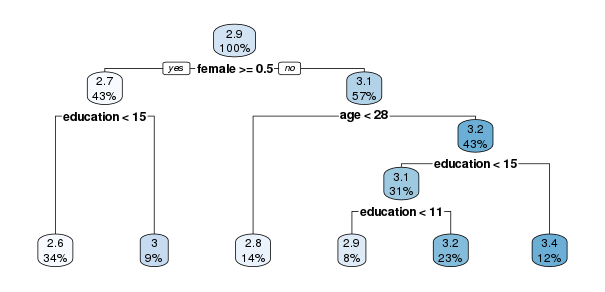
\includegraphics[width=\textwidth]{figures/Rpat1980_1985.png}
  \label{fig:decisiontree_1980_1985}
\end{figure}

\begin{figure}
  \centering
  \caption{Decision tree for real log wages, 2010-2016.}
  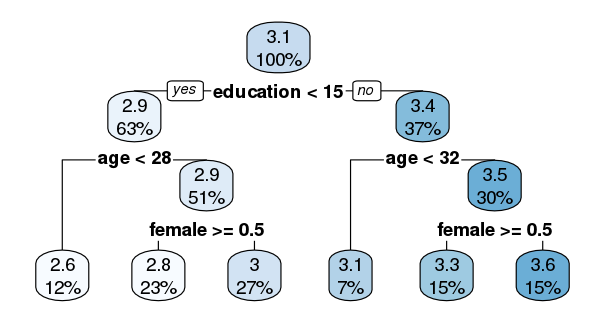
\includegraphics[width=\textwidth]{figures/Rpat2010_2016.png}
  \label{fig:decisiontree_2010_2016}
\end{figure}

Tree-based methods are a more modern approach to regression and prediction.  The process involves building a tree in the following process.  A data set of interest is taken, with a variable to be predicted (called the \textit{response} variable) and a number of variables used to predict it (called the \textit{predictor} variables).  A set of algorithms is applied to the data set, where an error function is minimised (similar to the OLS framework) for a defined amount of decisions that predict the response variable.  The decisions take the form of a true-false condition on given variables, leading to a final prediction conditional on all the given conditions.  Many methods involve using one data set or a subsample of a dataset as a \textit{training} sample, where a model is built (also called \textit{trained}) on the training set before being applied to a \textit{test} sample or new dataset to form predictions.

Figure~\ref{fig:decisiontree_1980_1985} presents a decision tree to depict such a model for log wages 1980--1985, figure~\ref{fig:decisiontree_2010_2016} for 2010--2016.  The regression tree approach allows for non-linearities and interactions between variables.  For the first tree, a woman with less than 15 years of education is predicted a log hourly wage of 2.6, a man over the age of 28 with more than 15 years of education is predicted 3.4.  The second tree predicts a log wage of 2.6 for someone who has less than 15 years of education and is younger than 28, 3.1 for someone with more than 15 years of education who is younger than 32.

The decision tree method generally over-fits its training data, making for a model which is not generalisable for a new data set or, indeed, the entire population.  A random forest approach builds many, many trees using random samples of the entire data set\footnote{This process is called bootstrapping, where at each step of the process a sample (with replacement) of the data set is taken.} as training sets and cross-validating across the sample,\footnote{Cross validation is a method to chose best value of parameter in cost function minimisation, a technical detail in building the prediction model.} making for a model which is less likely to over-fit the training data set.  This model specifically uses observations left out by sampling methods at each formed tree to form an estimate of the accuracy and so select technical parameters to maximise prediction accuracy.  The approach makes a model extremely good at capturing non-linearities and interactions in given data, to form a method extremely good at predicting a response variable.  Such non-linearities are displayed in Figures 3 and 4, where splitting according to specific variables -- and possibly multiple times in the same variable -- produces predictions, with no specific conditions or linearities needed.

It is important to be careful about predictor variable selection.  For example, hourly wage rate can be extremely well predicted by annual income.  However, this prediction process has no economic significance above demonstrating the well-known fact that annual income and hourly wage are very, very highly correlated.  \cite{mullainathan2017machine} note this issue of self-prediction and others in the use of big-data practices in economics.  The variables selected for random forest prediction are all the variables in the March CPS that have plausible causative relationships with income across the population.  They are as follows: age, gender, race, marriage status, dummies for living in a rural area, suburb, central city, whether they are self employed, union membership and total years of education.\footnote{The March CPS uniform extracts start with 475 variables, most of which are sub-variables not useful in this project.  These nine variables are those available for every year and that fit the plausible causative relationship criterion while also not causing any self-prediction problems.}$^{,}$\footnote{Missing values are coded as 0 to be included in tree prediction.  This transformation has no numerical effect in the tree-based methods other than ensuring they may be included in the analysis, and there are no missing values in variables used in OLS prediction.}  Work experience or a direct measure of potential experience is not available, so that selection on the age variable may indicate selection for experience in the same way that age is used as a measure of potential experience in a standard Mincer wage equation.

\subsection{Residuals in Wage Inequality}
Table~\ref{tab:inequalitymeasures} documents the distribution of residuals in five year groupings for 1980--2016,\footnote{6 year grouping for 2010--2016.} for the prediction methods: standard Mincer equation, adjusted Mincer equation, random forest prediction.  The standard deviation of the generated residuals is shown, as well as differences between the 90th and 10th, 90th and 50th, 50th and 10th percentiles.
\begin{table}[h]
\centering
\caption{Inequality Measures Based on Regression Model Residuals for Hourly Wage}
\label{tab:inequalitymeasures}
\begin{tabular}{@{\extracolsep{5pt}}ll|ccccccc} 
\\[-1.8ex]\hline 
\hline \\[-1.8ex] 
 & & 1980-- & 1985-- & 1990-- & 1995-- & 2000-- & 2005-- & 2010-- \\
\hline \\[-1.8ex] 
  Mincer & S.d. & 0.46 & 0.47 & 0.47 & 0.51 & 0.53 & 0.54 & 0.54 \\ 
   & 90-10 & 1.17 & 1.18 & 1.18 & 1.22 & 1.26 & 1.28 & 1.30 \\ 
   & 90-50 & 0.61 & 0.60 & 0.60 & 0.64 & 0.66 & 0.68 & 0.70 \\ 
   & 50-10 & 0.56 & 0.57 & 0.58 & 0.59 & 0.60 & 0.60 & 0.60 \\ \hline \\[-1.8ex] 
  Mincer, & S.d. & 0.46 & 0.47 & 0.47 & 0.51 & 0.53 & 0.53 & 0.54 \\
  adjusted & 90-10 & 1.17 & 1.18 & 1.18 & 1.21 & 1.25 & 1.26 & 1.29 \\ 
   & 90-50 & 0.61 & 0.60 & 0.60 & 0.63 & 0.66 & 0.67 & 0.70 \\ 
   & 50-10 & 0.56 & 0.57 & 0.58 & 0.58 & 0.59 & 0.59 & 0.59 \\ \hline \\[-1.8ex] 
  Random & S.d. & 0.41 & 0.43 & 0.44 & 0.48 & 0.50 & 0.51 & 0.52 \\ 
  forest & 90-10 & 1.00 & 1.05 & 1.08 & 1.13 & 1.16 & 1.18 & 1.22 \\ 
   & 90-50 & 0.52 & 0.53 & 0.54 & 0.58 & 0.61 & 0.62 & 0.65 \\ 
   & 50-10 & 0.49 & 0.52 & 0.53 & 0.54 & 0.55 & 0.55 & 0.57 \\ \hline \\[-1.8ex] 
  \multicolumn{2}{l}{Observations:}  & 275,813 & 266,275 & 271,907 & 247,343 & 341,165 & 308,241 & 474,776 \\ 
\hline 
\hline \\[-1.8ex] 
\end{tabular} 
\end{table}

The standard deviation for all models increases across the the 36 year period, being similar for the 1980--1984 grouping.  Interestingly, both forms of the Mincer equation return a nearly identical distribution of residuals, increasing from 0.46 to 0.52 while the random forest prediction gives slightly lower (yet similar) values.  The 90-10 percentile differential generally increases across the groupings, showing a more unequal distribution  of residuals in later years.  The 90-50 and 50-10 percentile differentials also increase across the years, those this rise is not as pronounces as for the 90-10 differential.  

It makes sense for the random forest method to produce lower values for inequality across the residual distribution, as this modern prediction technique is generally more accurate in predictions, thus producing smaller errors/residuals.  This can be seen in a year-specific comparison of the coefficient of determination, $R_t^2$ for years $t=1980, 1981, \dots , 2007, 2009, \dots , 2016$:
\begin{equation}
R^2_t = 1 - \frac{\sum_{i=1}^n(Y_{it} -  \hat{Y}_{it})^2}{\sum_{i=1}^n (Y_{it} - \bar{Y}_{it})^2} = 1 - \frac{\sum_{i=1}^n\varepsilon_{it}^2}{\sum_{i=1}^n (Y_{it} - \bar{Y}_{it})^2}
\end{equation}

\begin{figure}[h]
  \caption{Coefficient of Determination by Prediction Model, 1980--2016}
  \centering
  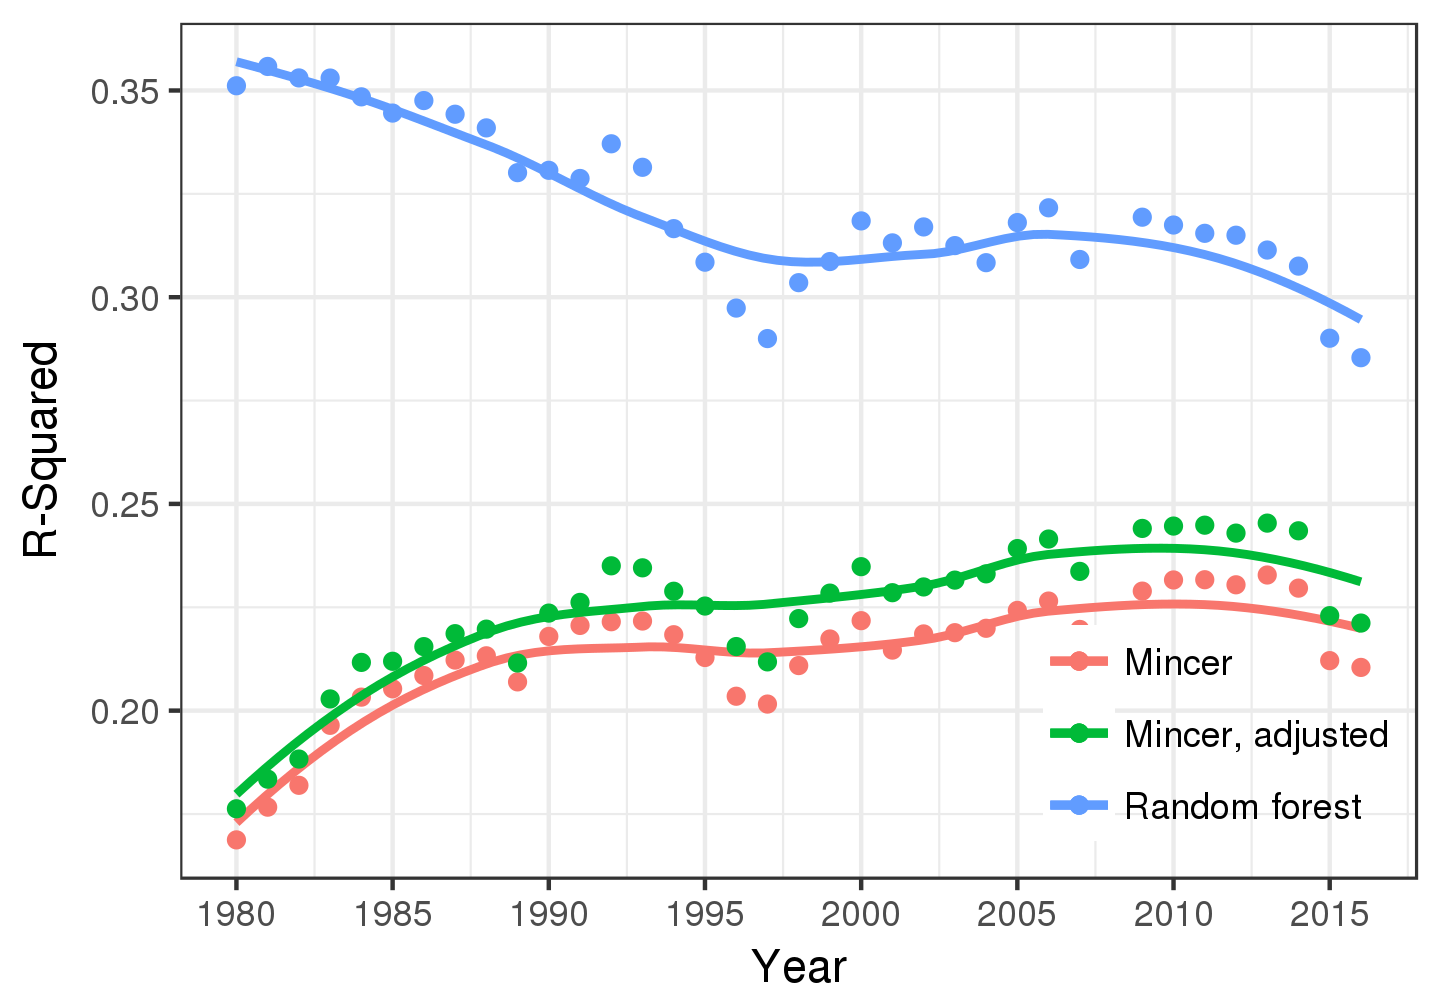
\includegraphics[width=0.65\textwidth]{figures/rsquared.png}
\end{figure}
\noindent
$R^2$ is consistently higher for random forest prediction than either form of the Mincer equation, as expected.  In 1980 the random forest has an associated $R_{1980}^2$ of 0.35, while the Mincer equation has 0.14 and 0.15 for the adjusted form.  The $R_t^2$ for both forms of Mincer equation rises to around 0.2 in 1985, before staying between 0.2 and 0.25 for the remaining years.  The random forest's $R^2_t$ drops to around 0.3 in 1995, before staying around this value for the following years.

% RESULTS
\section{Results}
\label{results}

\begin{table}[h!]
\centering
\caption{Mincer Wage Equation Results}
\label{tab:mincerresults}
\begin{tabular}{@{\extracolsep{5pt}}lcc} 
\\[-1.8ex]\hline 
\hline \\[-1.8ex] 
 & \multicolumn{2}{c}{\textit{Dependent variable:}} \\ 
\cline{2-3} 
\\[-1.8ex] & Log hourly wage & Log annual income \\ 
\\[-1.8ex] & (1) & (2)\\ 
\hline \\[-1.8ex] 
 Years education & 0.090$^{***}$ & 0.104$^{***}$ \\ 
  & (0.0001) & (0.0002) \\ 
  Potential experience & 0.032$^{***}$ & 0.057$^{***}$ \\ 
  & (0.0001) & (0.0001) \\ 
  (Potential experience)$^2$ & $-$0.001$^{***}$ & $-$0.001$^{***}$ \\ 
  & (0.00000) & (0.00000) \\ 
  Constant & 1.392$^{***}$ & 8.511$^{***}$ \\ 
  & (0.002) & (0.003) \\ 
 \hline \\[-1.8ex] 
Observations & 2,185,520 & 2,185,520 \\ 
$R^{2}$ & 0.222 & 0.230 \\
\hline 
\hline \\[-1.8ex] 
\textit{Note:}  & \multicolumn{2}{r}{$^{*}$p$<$0.1; $^{**}$p$<$0.05; $^{***}$p$<$0.01} \\ 
\end{tabular} 
\end{table}
Table~\ref{tab:mincerresults} presents the results of a standard Mincer equation in predicting wages across the entire sample period (i.e. estimating the regression with fixed coefficients $\bar{\beta}$).  The returns to education are fairly standard, at around 9 to 10\% increase for an additional year of education, with a significant and negative coefficient for the quadratic term of potential experience.  The $R^2$ value in both measures of income shows how this model captures around 22\% of the variation in wages for the entire sample period.

\begin{figure}[h]
  \centering
  \begin{subfigure}{.5\textwidth}
    \centering
    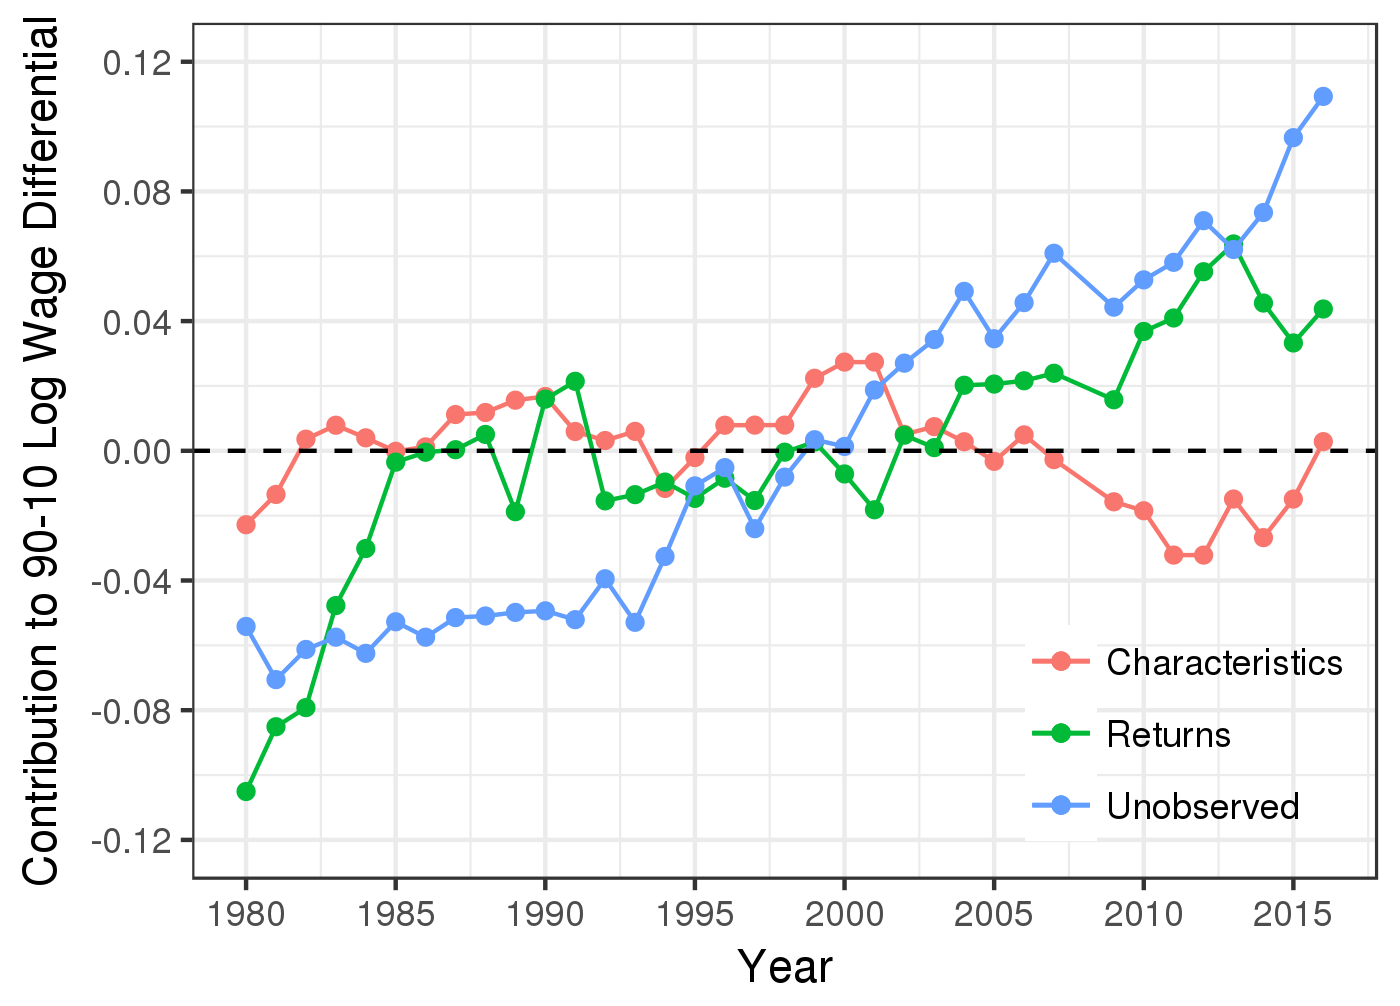
\includegraphics[width=\textwidth, height = 0.8\textwidth]{figures/edit1.png}
    \caption{Standard Mincer Equation}
  \end{subfigure}%
  \begin{subfigure}{.5\textwidth}
    \centering
    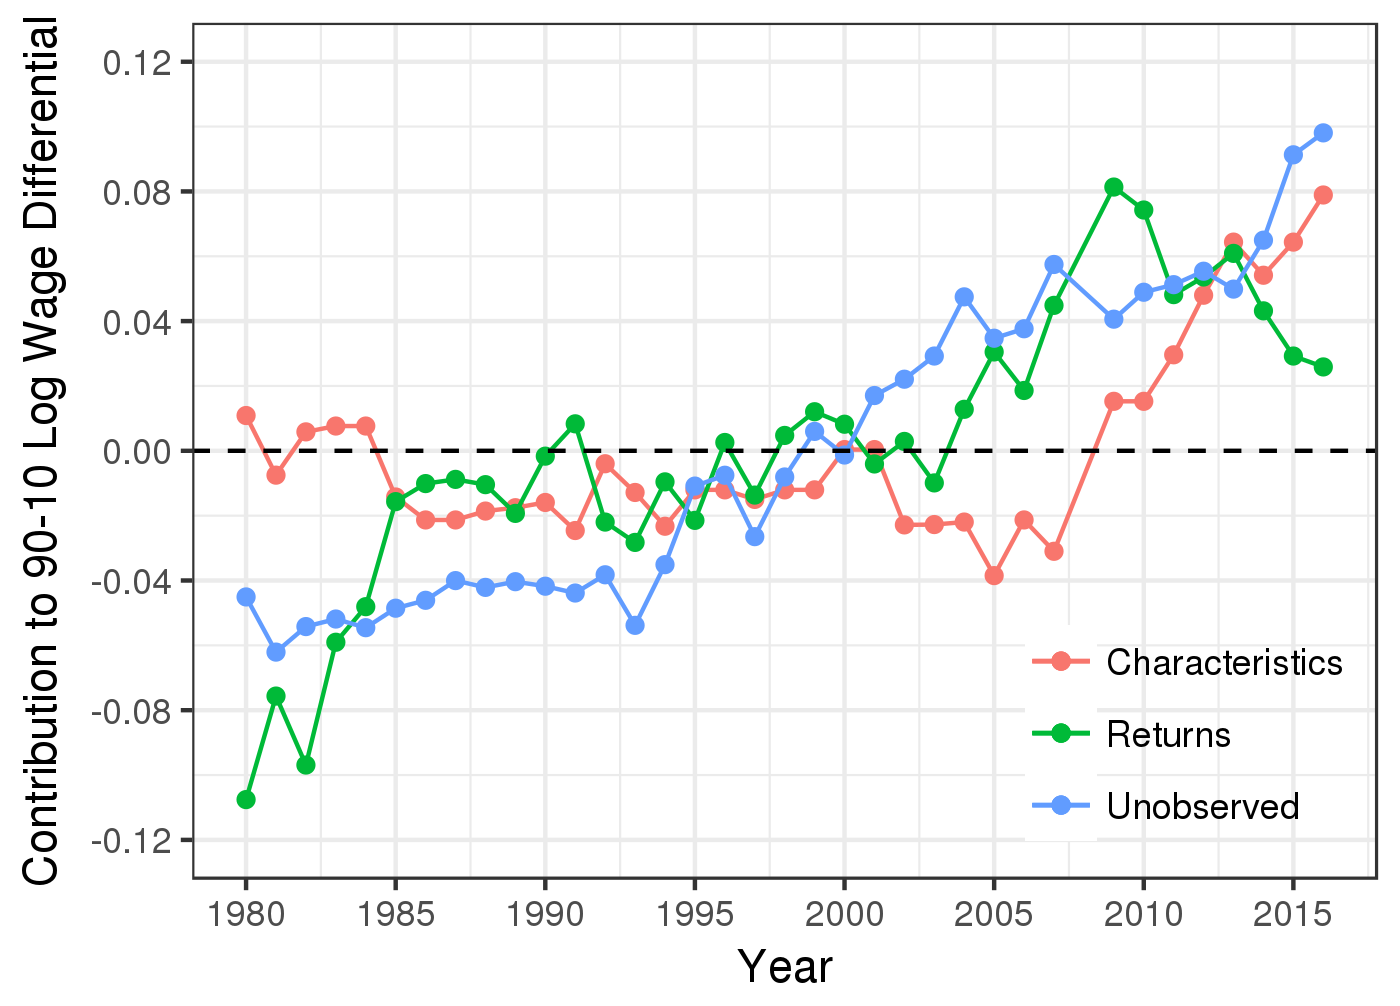
\includegraphics[width=\textwidth, height = 0.8\textwidth]{figures/edit2.png}
    \caption{Adjusted Mincer Equation}
  \end{subfigure}
  \caption{Components of 90-10th Log Hourly Wage Percentile, 1980--2016}
  \label{fig:components_regression}
\end{figure}

\begin{figure}[htb!]
  \centering
  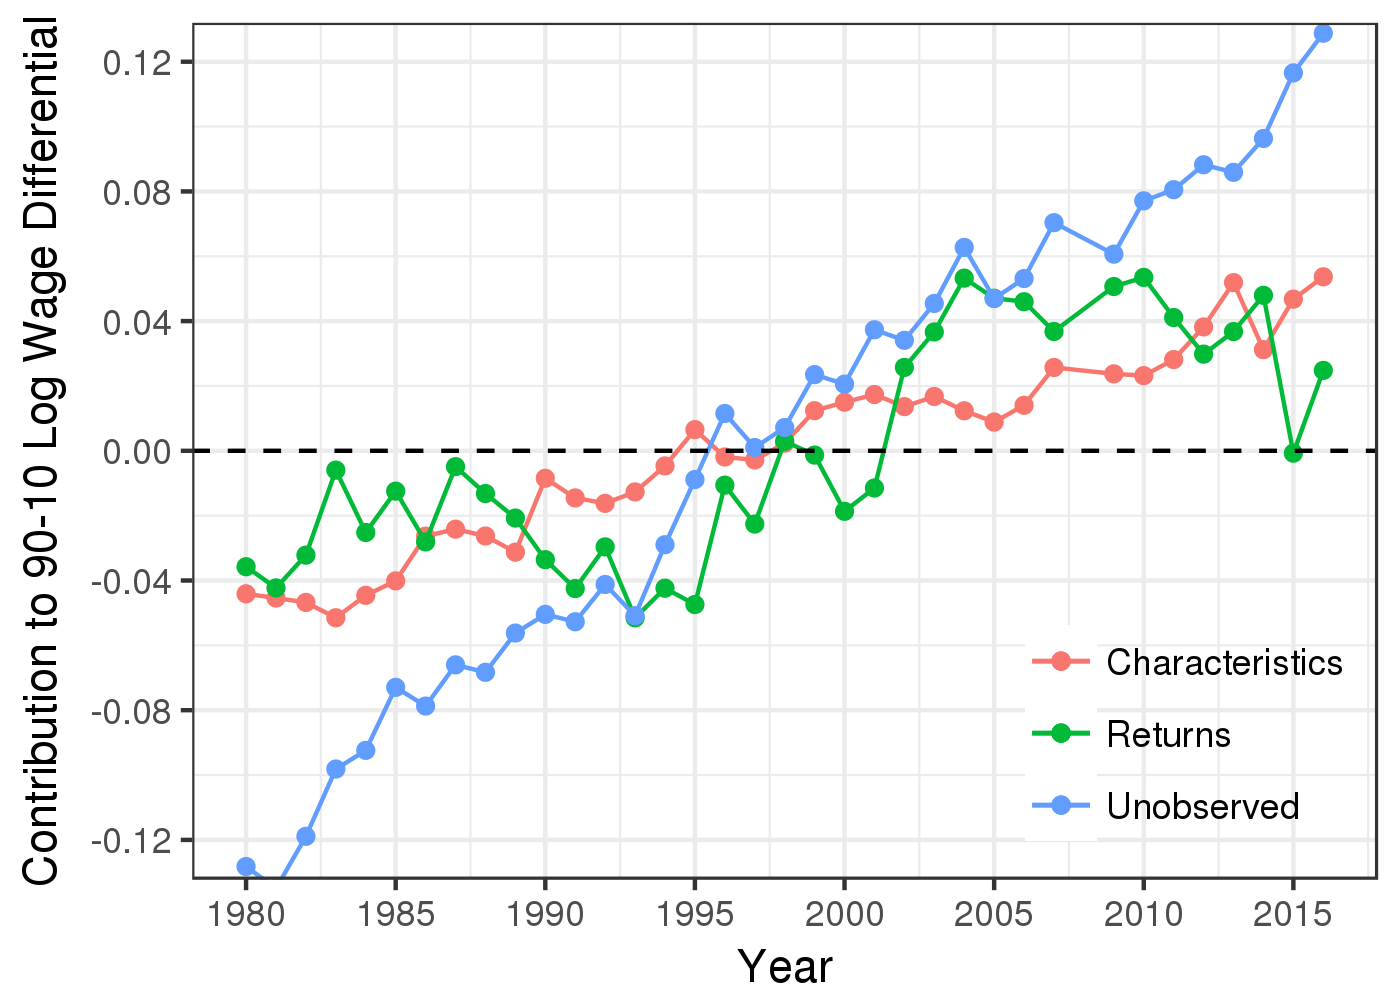
\includegraphics[width=0.7\textwidth]{figures/edit3.png}
  \caption{Components of 90-10th Log Hourly Wage Percentile for Random Forest Prediction, 1980--2016}
  \label{fig:components_randomforest}
\end{figure}

Figures~\ref{fig:components_regression} and \ref{fig:components_randomforest} give the components of the 90-10th percentile log wage differential accounted for by the three components by each prediction method, minus their mean.\footnote{Components do not sum to 1 as the graphs show change over time.}$^{,}$\footnote{The 90-10th percentile log wage differential is mathematically identical to the 90-10 wage ratio, so that the components contribute to the figures in Figure~\ref{fig:wages_percentile}.}  In every instance, unobserved characteristics rise more than any other component in the contribution to the wage differential.  The Mincer regressions are similar in their decomposition of components, simulating a similar and significant rise in the component of unobserved characteristics.  The contribution of observed characteristics doesn't change drastically, except for the adjusted form for after 2005 where the contribution rises significantly.  Returns to observed characteristics rise rapidly 1980--1990 in the standard Mincer regression,\footnote{An almost exact replication of the trend by \cite{juhn1993wage}, as expected.} with a very similar profile for the adjusted equation.  After 1990 returns to observed characteristics do not continue on the same rapid increase in either regression, though do follow a broad increase in contribution.

The decomposition using random forest prediction differs markedly from the Mincer decompositions in the component change for observed characteristics.  There is a steady rise over the entire time period of the role of observed characteristics in contributing to the wage differential, disagreeing completely with the standard regression's components.  Returns to observable skill follow a similarly stagnant path before rising in contribution in the 2000s.  And lastly, the contribution of unobserved characteristic and returns rises consistently and more significantly than in any other prediction method.
\begin{table}[h]
\centering
\caption{Observed and Unobserved Components of Changes in Inequality 1980--2016}
\label{tab:components}
\begin{tabular}{@{\extracolsep{5pt}}lr|ccccccc} 
\\[-1.8ex]\hline 
\hline \\[-1.8ex] 
 & Differential & Total & Observed & Observed & Unobserved  \\
  & & Change & Quantities & Prices & Differences  \\
 & & (1) & (2) & (3) & (4) \\
\hline \hline \\[-1.8ex] 
 Mincer & \\
 & 90-10 &  0.264 & 0.006 & 0.049 &  0.147 \\ 
   & 90-50 &  0.193 & 0.027 & 0.020 &  0.103 \\ 
   & 50-10 &  0.070 &  -0.021 & 0.029 &  0.043 \\
  \\[-1.8ex] \hline
 Mincer, & \\
 adjusted &  90-10 &  0.264 &  0.065 & 0.067 &  0.132 \\ 
   & 90-50 &  0.193 &  0.013 & 0.024 &  0.100 \\ 
   & 50-10 &  0.070 &  -0.052 & 0.042 &  0.032 \\
 \\[-1.8ex] \hline
 Random & \\ 
 forest & 90-10 &  0.264 &  0.091 & -0.043 &  0.229 \\ 
  & 90-50 &  0.193 &  0.044 & -0.018 &  0.148 \\ 
  & 50-10 &  0.070 &  -0.047 & 0.024 &  0.081 \\
\hline 
\hline  \\[-1.8ex] 
\end{tabular} 
\end{table}

Table~\ref{tab:components} presents the total change in the log wage differential for 1980--2016,\footnote{Again using 3 year groups to minimise small-sample variation.} with contribution of each component.  The components in columns 2--3 theoretically sum to the total change in column 1 yet there is some error in practice, yielding non-perfect sums as noted by \cite{autor200914}.  Unobserved characteristics is the largest component for all prediction techniques, but is estimated to be a much larger component in random forest prediction than in the others.  The Mincer equations estimate change in observed prices as the second biggest component to the wage differential, while observed quantities barely contributing.  The role is reversed in random forest prediction, where observed returns even contributing negatively to the wage differential i.e. the conterfactual distribution of wages under varying returns is estimated to have a \textit{lower} wage differential in 2016 than in 1980 -- which is clearly not observed.

Figure~\ref{fig:variableimportance} documents variable importance in random forest prediction of log hourly wages for the three variables which were most important: age, years of education and gender.  Age is likely selected on so frequently because of its high correlation with experience in the work force so that older workers have higher wages.  Over the sample period the role of education in predicting wages increases, shown a trend line, while the role of age stays constant and gender falls.  This result supports findings that estimate a rising role of returns to observable characteristics over the sample period.  This graph also gives a representation of the diminishing role of gender in determining wages, or in other words, the decrease (though not disappearance) of large wage differences between male and female wages.
\begin{figure}[H]
  \centering
  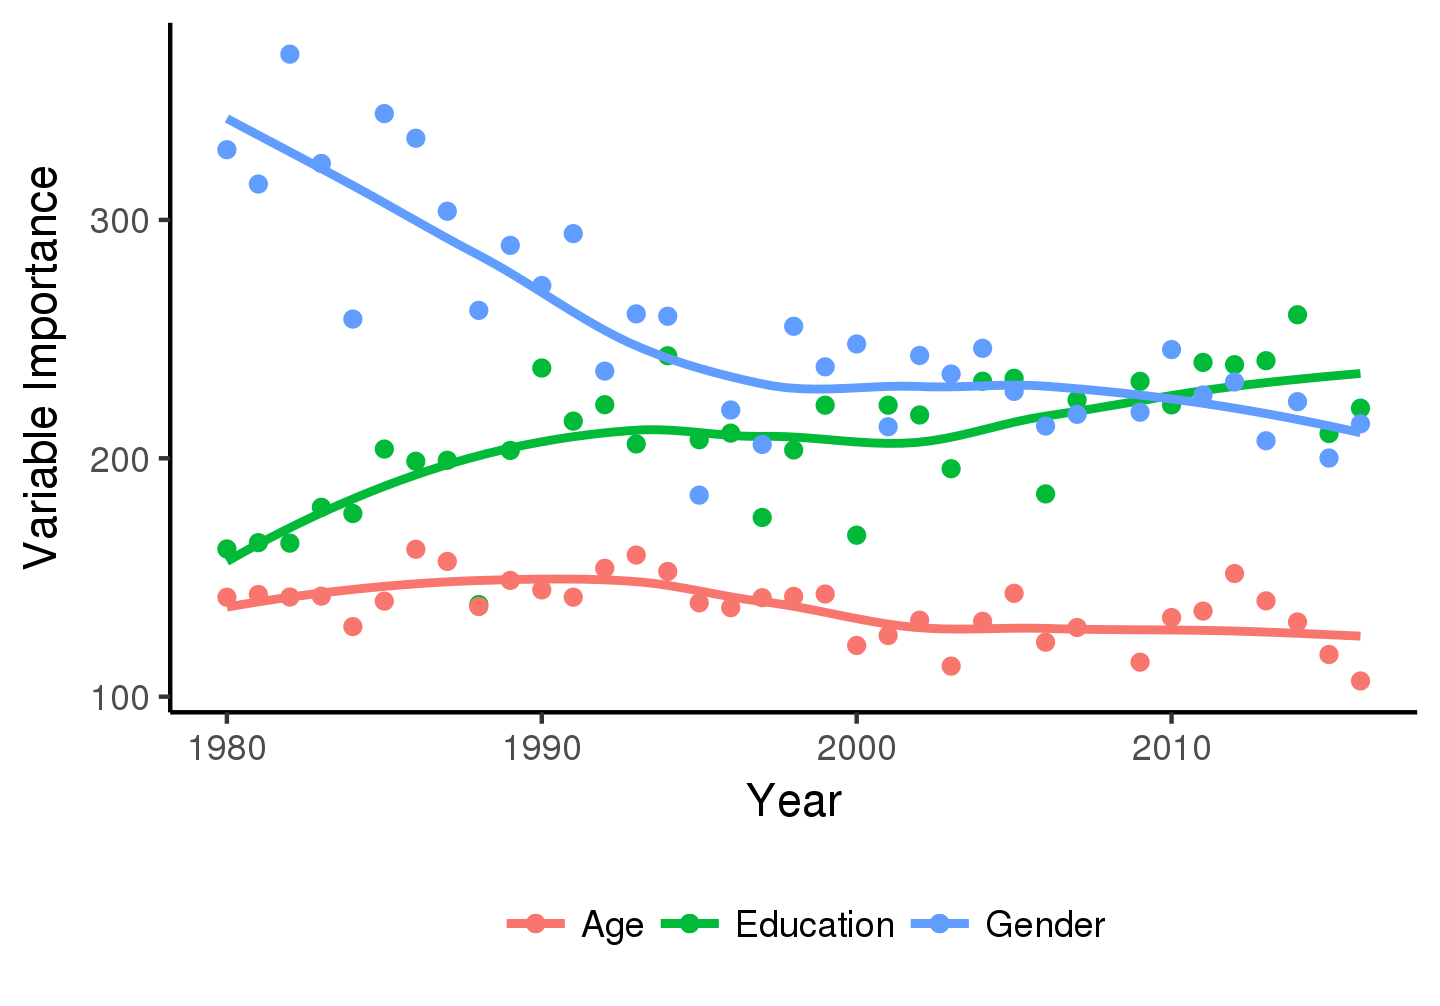
\includegraphics[width=0.8\textwidth]{figures/importance_graph.png}
  \caption{Variable Importance in Random Forest Prediction, 1980--2016}
  \label{fig:variableimportance}
\end{figure}

% DISCUSSION
\section{Discussion and Limitations}
\label{discussion}
This paper provides estimates for a greater role of unobserved skill in explaining rising inequality for 1980 and onwards than has been estimated in previous years.  This reinforces the interpretation of \cite{juhn1993wage} of the rise in returns to unobserved skill before 1985, extending the same findings and interpretation to 2016.  The role of unobserved skill in explaining rising inequality seems to be even higher today than it was before 1985, when estimated by standard linear regressions and even more so with modern regression techniques.  There are many possible interpretations of these findings.  Modern prediction methods better use given data and characteristics to predict wages, so that if they cannot attribute much of the rise in inequality to any of these observed returns or characteristics, then they attribute an even greater component of inequality to unobserved characteristics.  It follows that even with more covariates, and more efficient use of them, the rise in wage inequality is even less explainable than was previously estimated in labour economics.

This analysis has focused on the use of different prediction models in an extremely famous decomposition of wages and wage inequality.  The decomposition method was, of course, built to consider a linear regression in prediction methods.  The exact equation for the procedure in section reflects this, exampling the novel process of applying other prediction methods to this decomposition.  The comparison across models leads to the question: which prediction models provide the correct estimate for the role of the components in explaining rising wage inequality? 


Standard econometric methods in the ordinary least framework have decades and decades of research and analysis depicting their mathematical properties.  These properties range from simple consistency, unbiasedness in the Guass-Markov theorem to numerous important and more complicated properties.  Modern prediction methods are extremely good at predicting variables, even only using variables determined to have economic significance.  They do not, however, have the same research on their exact statistical properties.  For example, consider the property of consistency.  This means that asymptotically a parameter estimator converges in probability  to its true value, and has a short proof for a standard OLS regression under some standard assumptions.  It's not so clear what form this property even takes in modern regression techniques,\footnote{For example in a random, is that forming the optimal number of splits in variables, optimal number of bootstrapped trees, or whatever leads to the best predictions?} let alone what conditions must be satisfied for it to apply.

Modern regression techniques, including random forests, are designed to (and successfully do) produce better estimates for response variables with computational algorithms, but they can use any number of variables to predict other variables.  This is commonly called data-mining, where any data can be found to have some form of statistical pattern to predict a response variable though the process may have no economic intuitive or interpretable significance.  This issue has been addressed in these methods by using a well-defined set of intuitive and economically significant variables to predict wages (and avoiding self-prediction).  Future research on using computational statistics in economic research will need to address the question of what should be considered predictor variables -- the same as choosing what should be considered observable characteristics in this paper.  If we can one day collect so many more variables on people that have reasonable causative relationship for wages, should they all be considered observable characteristics?  If not, then is the line drawn at only observing gender, years of education and potential experience as in the Mincer wage equation?

The random forest method was chosen as one of the best prediction methods that is easily reproducible in standard statistical software that also has a fairly intuitive basis for understanding.  The field of computational statistics and machine learning is progressing extremely fast, so that newer or adjusted prediction methods with better accuracy are already available.  This means that the statistical methods of elaborating wage decompositions to tree-based methods is only scratching the surface of using new modern prediction methods beyond a linear regression framework in these methods.

% Conclusion
\section{Conclusion}
\label{conclusion}
This analysis documented a rise in wage inequality for 1980--2016, continuing the well-documented rise for 1960--1980.  The trend to greater inequality is attributed to a rise in returns to skill, observed (such as education and experience) and unobserved.  Modern prediction techniques attribute the rise in inequality even more so to unobserved characteristics than standard linear models, exhibiting the dependence of the \cite{juhn1993wage} decomposition method to specific prediction methods.  Specifically, random forest estimates that observed characteristics have contributed steadily more to inequality since 1980, and unobserved characteristics and returns have increased at a significantly higher rate.  Furthermore, years of education is increasingly important in predicting wages, supporting the interpretation that rise in returns to observed skill have also steadily risen.

It in unclear in this wage decomposition where the role of other factors than the three components identified fit in.  For example, recent research has concentrated on the role of constrained competition and rising barriers to entry in rising inequality in the US.  Perhaps this factor fits in to unobserved skill, or to observed skill for those with higher education and positions in concentrated industries or large companies.  Future research on the components of rising inequality at the individual level may need to provide a greater framework to consider such larger scale issues.

The basic rationale for the rise in returns to observable skill is the growth for demand for highly skilled workers and skill-biased technological change.  However, there is no consensus for what is driving an increase in the role of unobserved characteristics and returns in explaining wage inequality. The modern prediction methods provide better estimates for wages than standard econometric methods, but attribute the rise in inequality more to what is unobserved than in previous research.  Future research on the role of unobserved and observed skill in determining the level of inequality in the US -- as well as all economic research that uses or has used standard linear models for prediction purposes -- requires more attention to the choice of prediction methods used.

\bibliographystyle{agsm}
\bibliography{bibliography}
\end{document}
